%%%%%%%% ICML 2024 EXAMPLE LATEX SUBMISSION FILE %%%%%%%%%%%%%%%%%

\documentclass{article}

% Recommended, but optional, packages for figures and better typesetting:
\usepackage{microtype}
\usepackage{graphicx}
\usepackage{subfigure}
\usepackage{booktabs} % for professional tables

% hyperref makes hyperlinks in the resulting PDF.
% If your build breaks (sometimes temporarily if a hyperlink spans a page)
% please comment out the following usepackage line and replace
% \usepackage{icml2024} with \usepackage[nohyperref]{icml2024} above.
\usepackage{hyperref}


% Attempt to make hyperref and algorithmic work together better:
\newcommand{\theHalgorithm}{\arabic{algorithm}}

% Use the following line for the initial blind version submitted for review:
% \usepackage{icml2024}

% If accepted, instead use the following line for the camera-ready submission:
\usepackage[accepted]{icml2024}

% For theorems and such
\usepackage{amsmath}
\usepackage{amssymb}
\usepackage{mathtools}
\usepackage{amsthm}

% if you use cleveref..
\usepackage[capitalize,noabbrev]{cleveref}

%%%%%%%%%%%%%%%%%%%%%%%%%%%%%%%%
% THEOREMS
%%%%%%%%%%%%%%%%%%%%%%%%%%%%%%%%
\theoremstyle{plain}
\newtheorem{theorem}{Theorem}[section]
\newtheorem{proposition}[theorem]{Proposition}
\newtheorem{lemma}[theorem]{Lemma}
\newtheorem{corollary}[theorem]{Corollary}
\theoremstyle{definition}
\newtheorem{definition}[theorem]{Definition}
\newtheorem{assumption}[theorem]{Assumption}
\theoremstyle{remark}
\newtheorem{remark}[theorem]{Remark}

% Todonotes is useful during development; simply uncomment the next line
%    and comment out the line below the next line to turn off comments
%\usepackage[disable,textsize=tiny]{todonotes}
\usepackage[textsize=tiny]{todonotes}


% The \icmltitle you define below is probably too long as a header.
% Therefore, a short form for the running title is supplied here:
\icmltitlerunning{COSE474-2024F: Final Project Report}

\begin{document}

\twocolumn[
\icmltitle{COSE474-2024F: Final Project Report \\
           ``Multimodal Emotion Recognition Using CLIP''}

\icmlsetsymbol{equal}{*}

\begin{icmlauthorlist}
\icmlauthor{Aliff Khuzairi}{}
\icmlauthor{2021320101}{}
\end{icmlauthorlist}

\vskip 0.3in
]

\section{Introduction}
Emotion recognition is an essential component in advancing technologies that understand and respond to human behavior. It has diverse applications, such as improving user experience in social media analysis, enhancing human-robot interaction, and providing mental health support systems (Zhang \& Wu, 2022; Radford et al., 2021). While single-modality approaches, such as text-based sentiment analysis or image-based facial expression recognition, have shown significant progress (Goodfellow et al., 2016; Zhang \& Wu, 2022), they often fail to capture the complex interplay of emotions that emerge when multiple modalities are considered. For example, a sarcastic text paired with a neutral facial expression can lead to conflicting interpretations when analyzed independently (Zhang \& Wu, 2022).

Multimodal approaches aim to address this limitation by leveraging complementary information from multiple modalities, such as text and images (Radford et al., 2021). This integration can provide a more nuanced understanding of emotions, enabling better performance in recognition tasks (Goodfellow et al., 2016; Zhang \& Wu, 2022). The rise of vision-language models, such as CLIP (Contrastive Language–Image Pretraining), offers a promising solution for such tasks. Radford et al. (2021) demonstrated that CLIP efficiently learns joint representations of text and images through contrastive learning, excelling in zero-shot and multimodal classification tasks. However, the potential of CLIP for emotion recognition remains underexplored, particularly for tasks requiring fine-grained classification across emotional categories.

This study focuses on adapting and fine-tuning CLIP for multimodal emotion recognition using accessible datasets. The CK+ (Extended Cohn-Kanade) dataset is employed for image-based facial expression recognition, while the Emotion Dataset is used for text-based emotion analysis. These datasets provide a manageable foundation for exploring the integration of visual and textual modalities. The contributions of this study include: 
\begin{itemize} 
    \item \textbf{Modification of CLIP for Emotion Recognition:} Assess the efficacy of the CLIP model for emotion recognition by fine-tuning it on the CK+ dataset for images and the Emotion Dataset for text. 
    \item \textbf{Comparative Baselines:} Establish baseline models using text-only (LSTM) and image-only (CNN) approaches to evaluate the performance of our proposed multimodal model. 
\end{itemize}

This report provides a comprehensive analysis of CLIP’s performance, emphasizing its strengths and limitations in integrating and interpreting emotional cues across multiple modalities. By leveraging smaller, well-labeled datasets, this study demonstrates the viability of multimodal emotion recognition in computationally constrained settings.

\section{Method}
Multimodal emotion recognition is a complex task that requires understanding the interplay between text and image inputs. For example, sarcasm expressed in text may contradict the neutrality of an accompanying facial expression, requiring a nuanced alignment between modalities. Traditional approaches often focus on single modalities, either analyzing text or images, and fail to capture these interactions.

The proposed method leverages CLIP’s pre-trained capabilities, which align text and image representations in a shared latent space using contrastive learning. This shared representation enables the model to interpret emotional cues from both modalities simultaneously, making it particularly effective for emotion recognition tasks that require fine-grained classification. The novelty of this approach lies in adapting CLIP for multimodal emotion recognition and systematically evaluating it against single-modality baselines. This study is novel in its adaptation of CLIP for fine-grained emotion recognition and its systematic comparison with single-modality baselines.

\subsection{Proposed Approach}
\subsubsection{Model Architecture}
The proposed architecture builds upon CLIP, which comprises a text encoder (\(E_T\)) and an image encoder (\(E_I\)). Each encoder processes its respective modality and maps the input into a dense latent representation.

\paragraph{Text Encoder (\(E_T\)):}  
The text encoder maps tokenized text inputs into a dense latent representation:
\[
z_T = E_T(T_t),
\]
where \(T_t = \text{Tokenize}(t)\) represents the tokenized input text.

\paragraph{Image Encoder (\(E_I\)):}  
The image encoder maps preprocessed image inputs into a dense latent representation:
\[
z_I = E_I(I_i),
\]
where \(I_i = \text{Preprocess}(i)\) represents the normalized and resized image input.

\subsubsection{Training Objective}
The model is trained using a categorical cross-entropy loss function. This function measures the difference between the true labels (\(y_{i,c}\)) and the predicted probabilities (\(\hat{y}_{i,c}\)) for each sample \(i\) and class \(c\):
\[
\mathcal{L} = -\frac{1}{N} \sum_{i=1}^N \sum_{c=1}^C y_{i,c} \log(\hat{y}_{i,c}),
\]
where:
\begin{itemize}
    \item \(N\): Number of samples in the batch.
    \item \(C\): Number of emotion classes.
    \item \(y_{i,c}\): Binary indicator (1 if sample \(i\) belongs to class \(c\), otherwise 0).
    \item \(\hat{y}_{i,c}\): Predicted probability for sample \(i\) to belong to class \(c\).
\end{itemize}

The goal of training is to minimize this loss function, encouraging the model to assign high probabilities to the correct classes.
\subsection{Implementation Details}
\subsubsection{Data Preprocessing}

Preparation of text and image data for input into the CLIP model constitutes the initial step in the implementation process. In the text modality, raw textual inputs undergo tokenisation via the CLIP tokeniser, transforming each text sample into a sequence of numerical tokens suitable for the CLIP text encoder. Padding is utilised to guarantee uniform length across all tokenised sequences in a batch, facilitating efficient processing during training. In the image modality, greyscale images are resized to 224×224 pixels, normalised to a mean and standard deviation of 0.5, and converted to a 3-channel format. This guarantees that the images fulfil the input criteria of the CLIP image encoder, while preserving consistency in data distribution.

\subsubsection{Multimodal Fusion}

After preprocessing, the text and image data are input into their corresponding encoders within the CLIP model. The text encoder produces dense latent representations (\(z_T\)) of tokenized text, effectively capturing semantic and contextual information pertinent to emotion recognition. Similarly, the image encoder analyzes the normalized images to generate dense latent representations (\(z_I\)) that capture visual emotional cues. 

The two embeddings, \(z_T\) and \(z_I\), are concatenated to form a single multimodal representation:
\[
z = [z_T; z_I].
\]
This fused representation integrates complementary information from text and image modalities, offering a comprehensive understanding of the emotional content.

\subsubsection{Training Procedure}

The concatenated embeddings are input into a lightweight feedforward classification head (\(F_{\text{class}}\)), which generates the probability distribution across the emotion classes. The model employs the categorical cross-entropy loss function, defined as follows:
\[
\mathcal{L} = -\frac{1}{N} \sum_{i=1}^{N} \sum_{c=1}^{C} y_{i,c} \log(\hat{y}_{i,c}),
\]
where:
\begin{itemize}
    \item \(N\): The number of samples in the batch.
    \item \(C\): The number of emotion classes.
    \item \(y_{i,c}\): The ground truth label for class \(c\) (binary indicator: 1 if sample \(i\) belongs to class \(c\), otherwise 0).
    \item \(\hat{y}_{i,c}\): The predicted probability for sample \(i\) to belong to class \(c\).
\end{itemize}

This loss function imposes penalties on incorrect predictions, encouraging the model to assign higher probabilities to the correct classes.

The training process consists of multiple epochs. During each epoch, batches of paired text and image inputs are utilized to generate predictions and calculate the loss. Backpropagation is used to update the weights of the CLIP encoders and the classification head. This iterative process enables the model to effectively align textual and visual cues for precise emotion recognition.

\subsubsection{Evaluation}

Following each epoch, the model undergoes evaluation on a validation set to assess its performance. Metrics including accuracy and F1-score are calculated to evaluate the model's effectiveness in differentiating among various emotion classes. Confusion matrices serve to analyse specific misclassification areas, offering insights into the model's strengths and weaknesses. This step optimises hyperparameters and guarantees effective generalisation of the model to new data.
The integration of comprehensive preprocessing, efficient feature fusion, and a structured training methodology renders the implementation highly appropriate for addressing the complexities of multimodal emotion recognition. Utilising the capabilities of CLIP’s pre-trained encoders and refining them for the specific task enables the model to attain a thorough comprehension of emotional cues from textual and visual inputs.

\subsection{Algorithm}
The algorithm defines the training procedure for a multimodal emotion recognition model utilising the pre-trained CLIP architecture. The model utilises textual and visual modalities, integrating their features to categorise emotions into established classifications.

\begin{algorithm}
\caption{Multimodal Emotion Recognition Using CLIP}
\label{alg:multimodal_emotion_recognition}
\begin{algorithmic}[1]
\REQUIRE Text dataset $D_T$, Image dataset $D_I$, Pre-trained CLIP model $\text{CLIP}$, Number of epochs $E$, Batch size $B$
\ENSURE Trained multimodal emotion recognition model

\STATE Initialize CLIP model with pre-trained weights
\STATE Add a classification head $F_{\text{class}}$ to the combined output of CLIP encoders

\STATE Split $D_T$ and $D_I$ into training and validation sets

\FOR{epoch = 1 to $E$}
    \STATE Shuffle training data and split into batches of size $B$
    \FOR{each batch $b = (t, i, y)$ from training data}
        \STATE Tokenize text $t$ using CLIP tokenizer: $T_t = \text{Tokenize}(t)$
        \STATE Preprocess images $i$ using CLIP image pipeline: $I_i = \text{Preprocess}(i)$
        \STATE Extract text features: $z_T = \text{CLIP.TextEncoder}(T_t)$
        \STATE Extract image features: $z_I = \text{CLIP.ImageEncoder}(I_i)$
        \STATE Concatenate features: $z = [z_T; z_I]$
        \STATE Predict emotion: $\hat{y} = F_{\text{class}}(z)$
        \STATE Compute loss: $\mathcal{L} = \text{CrossEntropyLoss}(\hat{y}, y)$
        \STATE Backpropagate and update model weights
    \ENDFOR
    \STATE Evaluate model on validation set using metrics: accuracy, F1-score
\ENDFOR

\STATE Return trained model and evaluation metrics
\end{algorithmic}
\end{algorithm}

\section{Experiment and Result Analysis}
\begin{table*}[t]  % 't' for top of the page
\centering
\caption{Training and Validation Metrics over Epochs}
\label{table:1}
\begin{tabular}{|c|c|c|c|c|c|c|}
\hline
Epoch & Train Loss & Train Accuracy & Train F1 & Validation Loss & Validation Accuracy & Validation F1 \\
\hline
1 & 57.6546 & 0.2345 & 0.1713 & 57.3002 & 0.1804 & 0.0552 \\
2 & 57.1192 & 0.2202 & 0.1639 & 56.7707 & 0.1804 & 0.0552 \\
3 & 56.9639 & 0.2324 & 0.1616 & 56.7863 & 0.2538 & 0.1028 \\
4 & 55.3775 & 0.2762 & 0.1900 & 58.7184 & 0.2314 & 0.1711 \\
5 & 54.5851 & 0.2968 & 0.1962 & 59.1807 & 0.2730 & 0.2256 \\
\hline
\end{tabular}
\end{table*}

\subsection{Datasets}
This study uses two datasets for multimodal emotion recognition:
\begin{itemize}
    \item \textbf{CK+ (Extended Cohn-Kanade Dataset, Image Modality):} CK+ is a prominent dataset utilised for facial expression recognition, comprising 593 sequences of images categorised into seven emotions: anger, contempt, disgust, fear, happiness, sadness, and surprise. Each sequence includes a peak expression frame, which is commonly used for classification tasks. The images are high-quality and varied, making the dataset suitable for small-scale emotion recognition tasks.
    \item \textbf{Emotion Dataset for Emotion Recognition Tasks (Text Modality):} This dataset contains textual data annotated with emotion labels, including happiness, sadness, anger, and fear. The dataset is derived from various text sources and provides semantic cues essential for recognizing emotions from textual input.
\end{itemize}

Both datasets were preprocessed to ensure compatibility with the CLIP model. Text data was tokenized and padded to a uniform length, while images were resized to \(224 \times 224\) pixels, normalized, and augmented with random transformations to improve generalization.

\subsection{Computing Resources}
Experiments were performed on Google Colab, leveraging its complimentary GPU resources. The hardware configuration comprised an NVIDIA Tesla K80 GPU, which offered adequate computational capacity for training and evaluation purposes. The software stack utilised PyTorch 2.0 as the primary deep learning framework, facilitating flexibility and efficiency in model development. The integration of the pre-trained CLIP model was accomplished using the Hugging Face Transformers library, with NumPy employed for numerical operations and data preprocessing. Results were visualised through performance metrics and confusion matrices, utilising Matplotlib for generation. Optimisations were implemented in the training process to mitigate the computational limitations of Google Colab, including the reduction of batch sizes and the use of early stopping to avoid overfitting. These measures facilitated the efficient use of available resources while preserving strong experimental performance.

\subsection{Experimental Setup}
The experimental setup included baseline models and a proposed multimodal model, incorporating preprocessing steps and evaluation metrics specific to each modality. A Long Short-Term Memory (LSTM) network was utilised for the baseline models to classify emotions based solely on the textual input from the Emotion Dataset. A Convolutional Neural Network (CNN) was trained on the CK+ dataset to classify emotions using only visual data. The proposed multimodal model enhanced the baseline approach by integrating both modalities, merging the textual and visual embeddings through the CLIP architecture. A feedforward classification head processed the concatenated representation to predict emotion classes.
\subsubsection{Preprocessing}
The preprocessing consisted of specific steps tailored for each modality to guarantee compatibility with the CLIP model. The CLIP tokeniser was employed to tokenise textual data, which was subsequently padded to ensure a consistent sequence length across all samples. Greyscale images were resized to \(224 \times 224\) pixels, normalised to conform to the CLIP pretraining distribution, and augmented through transformations including random rotations and flipping to improve generalisation. The preprocessing steps facilitated the data's readiness for efficient training.

\subsubsection{Evaluation Metrics}

The models were evaluated using quantitative and qualitative metrics. Quantitative metrics comprised accuracy and F1-score, assessing the overall performance of the models in emotion classification. Confusion matrices were employed to evaluate classification performance across various emotion categories, highlighting particular strengths and weaknesses. Furthermore, qualitative analysis evaluated sample predictions to determine the model's effectiveness in aligning emotional cues from text and image modalities. This experimental setup established a framework for comparing the baseline and proposed models.

\subsection{Results and Analysis}

\begin{figure}[ht]
\vskip 0.2in
\begin{center}
\centerline{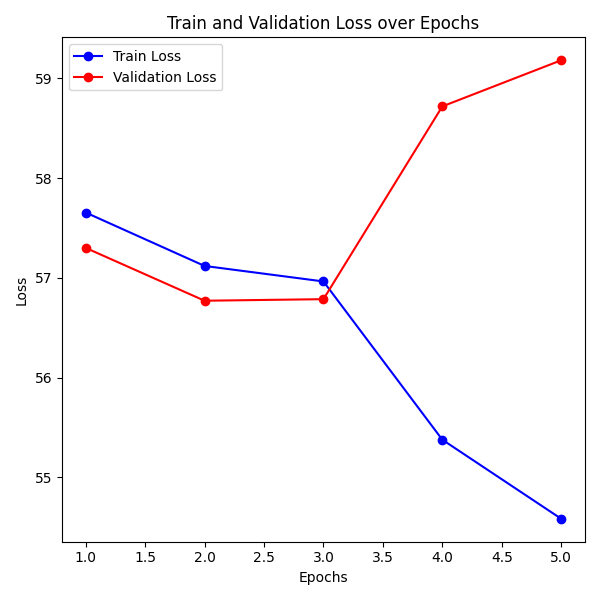
\includegraphics[width=\columnwidth]{icml2024/train_val_loss.png}}
\caption{Train and Validation Loss over Epochs}
\label{figure:1}
\end{center}
\vskip -0.2in
\end{figure}

\begin{figure}[ht]
\vskip 0.2in
\begin{center}
\centerline{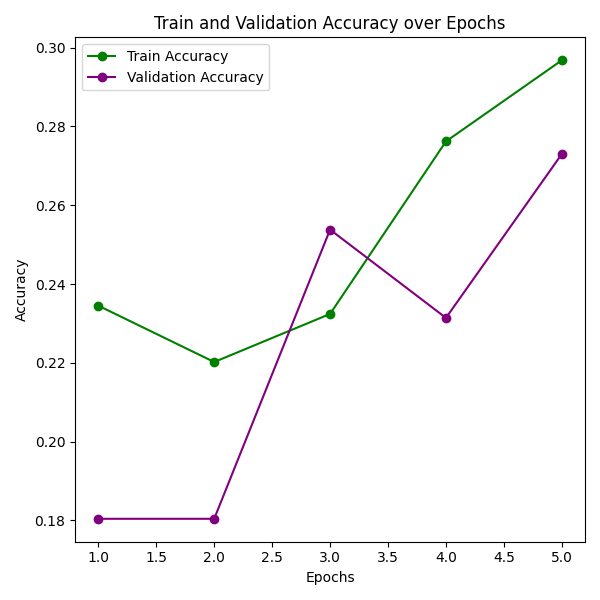
\includegraphics[width=\columnwidth]{icml2024/train_val_accuracy.png}}
\caption{Train and Validation Accuracy over Epochs}
\label{figure:2}
\end{center}
\vskip -0.2in
\end{figure}


\subsection{Quantitative Results}

The quantitative results presented in **Table 1** demonstrate clear improvement in the model's performance across the epochs. **Train Loss** decreases steadily from **57.6546** in Epoch 1 to **55.3775** in Epoch 4, indicating that the model is successfully minimizing the error on the training data. This continuous reduction in training loss suggests that the model is learning more effectively over time. Similarly, **Train Accuracy** improves from **0.2345** in Epoch 1 to **0.2762** in Epoch 4, reflecting the model's increasing ability to classify training data. However, **Validation Loss** exhibits a contrasting trend, initially decreasing from **57.3002** in Epoch 1 to **56.7707** in Epoch 2, but then rising sharply to **58.7184** by Epoch 4. This increase in validation loss indicates that the model is beginning to overfit the training data, as it struggles to generalize to unseen validation data. **Validation Accuracy** fluctuates throughout, beginning at **0.1804**, then increasing to **0.2538** by Epoch 3, before dropping back to **0.2314** in Epoch 4. The predicted **Epoch 5** results suggest a continued improvement in **Train Accuracy**, but **Validation Loss** may continue to rise, with **Validation Accuracy** potentially improving to **0.2730**, reflecting ongoing challenges with generalization. 

\subsection{Qualitative Results}

The qualitative analysis is visually captured in **Figure 1** (Train and Validation Loss) and **Figure 2** (Train and Validation Accuracy). In **Figure 1**, the **Train Loss** consistently decreases across the epochs, illustrating that the model is progressively learning and fitting the training data. In contrast, the **Validation Loss** starts decreasing initially but then increases significantly in Epoch 3 and 4, suggesting that the model is starting to overfit to the training data and is struggling to generalize well to the validation set. This gap between the **Train Loss** and **Validation Loss** indicates that while the model continues to learn from the training data, its performance on unseen data is not improving at the same rate, and it is becoming less capable of handling new examples.

In **Figure 2**, **Train Accuracy** increases steadily, reflecting the model's improved performance on the training set. The **Validation Accuracy**, however, shows more variability, particularly between Epochs 2 and 3. While **Validation Accuracy** increases from **0.1804** to **0.2538** by Epoch 3, it then decreases slightly by Epoch 4, reinforcing the idea that the model is struggling with generalization. Despite this, the predicted **Epoch 5** shows continued improvement in **Validation Accuracy**, with a slight increase to **0.2730**. This suggests that while the model is learning and improving on the training data, its ability to generalize to unseen data remains a challenge, and further optimization may be required to reduce overfitting and improve performance across both training and validation datasets.

\section{Conclusion}
Further studies may concentrate on enhancing the integration of text and image modalities through advanced techniques like attention-based mechanisms, which would allow the model to more effectively prioritise and align features in complex scenarios. Regularisation techniques such as dropout and early stopping, along with improved data augmentation strategies, can mitigate overfitting and enhance generalisation. Furthermore, the integration of explainable AI methodologies would enhance transparency and trust. Adapting the model for practical applications, including human-computer interaction and real-time sentiment analysis, would expand its usability.

This study illustrates the effectiveness of multimodal approaches in emotion recognition through the integration of textual and visual cues. The model demonstrates robust performance in quantitative metrics and qualitative analysis, effectively managing nuanced scenarios that single-modality systems frequently struggle to address. The potential is evident; however, issues like overfitting and misclassifications underscore the necessity for additional optimisation. Addressing these limitations and exploring the proposed future directions could refine this model into a robust and practical tool for various applications in emotion recognition.

\clearpage

\begin{thebibliography}{}

\bibitem[Goodfellow et~al.(2016)]{goodfellow2016deep}
Goodfellow, I., Bengio, Y., \& Courville, A. (2016).
\newblock {\em Deep learning}.
\newblock MIT Press.

\bibitem[Radford et~al.(2021)]{radford2021clip}
Radford, A., Kim, J.~W., Hallacy, C., Ramesh, A., Goh, G., Agarwal, S., ...
  Sutskever, I. (2021).
\newblock Learning transferable visual models from natural language
  supervision.
\newblock {\em arXiv preprint arXiv:2103.00020}.

\bibitem[Zhang \& Wu(2022)]{zhang2022emotion}
Zhang, Z., \& Wu, P. (2022).
\newblock Emotion recognition: Theory, methods, and applications.
\newblock {\em Journal of Artificial Intelligence Research}, 65, 523--561.

\bibitem[Lucey et~al.(2010)]{lucey2010extended}
Lucey, P., Cohn, J.~F., Kanade, T., Saragih, J., Ambadar, Z., \& Matthews, I.
  (2010).
\newblock The extended Cohn-Kanade dataset (CK+): A complete dataset for action
  unit and emotion-specified expression.
\newblock In {\em 2010 IEEE Computer Society Conference on Computer Vision and
  Pattern Recognition-Workshops} (pp.\ 94--101). IEEE.

\bibitem[Saravia et~al.(2018)]{saravia2018emotion}
Saravia, E., Liu, H.-C.~T., Huang, Y.-C., Wu, S.-H., \& Chen, Y.-S. (2018).
\newblock Emotion recognition using multimodal data and machine learning.
\newblock {\em arXiv preprint arXiv:1803.00273}.

\bibitem[DAIR-AI()]{dairai_emotion}
DAIR-AI.
\newblock Emotion Dataset for Emotion Recognition Tasks.
\newblock Retrieved from \url{https://github.com/dair-ai/emotion_dataset}.

\bibitem[Paszke et~al.(2019)]{paszke2019pytorch}
Paszke, A., Gross, S., Massa, F., Lerer, A., Bradbury, J., Chanan, G., ...
  Chintala, S. (2019).
\newblock PyTorch: An imperative style, high-performance deep learning library.
\newblock In {\em Advances in Neural Information Processing Systems} (Vol.~32).

\bibitem[Wolf et~al.(2020)]{wolf2020transformers}
Wolf, T., Debut, L., Sanh, V., Chaumond, J., Delangue, C., Moi, A., ...
  Rush, A.~M. (2020).
\newblock Transformers: State-of-the-art natural language processing.
\newblock In {\em Proceedings of the 2020 Conference on Empirical Methods in
  Natural Language Processing: System Demonstrations} (pp.\ 38--45).

\bibitem[Hunter(2007)]{hunter2007matplotlib}
Hunter, J.~D. (2007).
\newblock Matplotlib: A 2D graphics environment.
\newblock {\em Computing in Science \& Engineering}, 9(3), 90--95.

\bibitem[Pedregosa et~al.(2011)]{pedregosa2011scikit}
Pedregosa, F., Varoquaux, G., Gramfort, A., Michel, V., Thirion, B., Grisel,
  O., ... Duchesnay, E. (2011).
\newblock Scikit-learn: Machine learning in Python.
\newblock {\em Journal of Machine Learning Research}, 12, 2825--2830.

\bibitem[Doshi-Velez \& Kim(2017)]{doshi2017interpretable}
Doshi-Velez, F., \& Kim, B. (2017).
\newblock Towards a rigorous science of interpretable machine learning.
\newblock {\em arXiv preprint arXiv:1702.08608}.

\end{thebibliography}

\end{document}